\documentclass[conference]{IEEEtran}
\IEEEoverridecommandlockouts
% The preceding line is only needed to identify funding in the first footnote. If that is unneeded, please comment it out.
\usepackage{cite}
\usepackage{amsmath,amssymb,amsfonts}
\usepackage{algorithmic}
\usepackage{graphicx}
\usepackage{textcomp}
\usepackage{xcolor}
\def\BibTeX{{\rm B\kern-.05em{\sc i\kern-.025em b}\kern-.08em
    T\kern-.1667em\lower.7ex\hbox{E}\kern-.125emX}}
\begin{document}

\title{Hardware Accelerated Sorting\\
}

\author{\IEEEauthorblockN{1\textsuperscript{st} Omkar Madhukar Patil}
\IEEEauthorblockA{\textit{dept. of Electrical and} \\
\textit{Computer Engineering}\\
\textit{Stevens Institute of Technology}\\
Hoboken, USA \\
opatil@stevens.edu}
\and
\IEEEauthorblockN{2\textsuperscript{nd} Bradely O'Connell}
\IEEEauthorblockA{\textit{dept. of Electrical and} \\
\textit{Computer Engineering}\\
\textit{Stevens Institute of Technology}\\
Hoboken, USA \\
boconnell@stevens.edu}
\and
\IEEEauthorblockN{3\textsuperscript{rd} Nirmohi Samirbhai Patel}
\IEEEauthorblockA{\textit{dept. of Electrical and} \\
\textit{Computer Engineering}\\
\textit{Stevens Institute of Technology}\\
Hoboken, USA \\
npatel24@stevens.edu}
}

\maketitle

\begin{abstract}
 In this paper we proposed an implementation that optimizes hardware sorting. The sorting algorithm is guaranteed to provide the optimized result with less time. While much current hardware acceleration is focused on GPU compute, we applied a parallel sorting algorithm on FPGA to take advantage of its speed benefits. We have implemented Bitonic Merge Sort which functions parallel on FPGA decreasing the time complexity.
\end{abstract}

\begin{IEEEkeywords}
hardware acceleration, bitonic sort, parallel sorting, fpga
\end{IEEEkeywords}

\section{Introduction}
Sorting is foundational step in most of the applications which includes data, such as social networks, search, and data management (e.g. databases). Sorting can be done with various algorithms such as linear, parallel, divide and conquer, every algorithm having its own advantages. Some applications run sorting functions on hardware to get efficient outputs. Graphics Processing Units (GPU), Field Programmable Gate Arrays (FPGA) and Application-Specific Integrated Circuits (ASIC) are different hardware that can be programmed to perform sorting. Hardware accelerated sorting on GPU takes the msot time of these 3 devices. To reduce time complexity, this paper is focused on implementing the parellel sorting algorithm bitonic merge sort on an FPGA.

\section{Our Solution}

\subsection{Hardware}\label{AA}
For faster sorting we need hardware that helps parallel processing. FPGA and GPU both does parallel computing, but FPGAs are faster because they have more customized memory bandwidth where as due to multiple buffer memories GPUs delays the output. Also, FPGA provide customized ingress and egress, GPU does not provide that feature. During research we found that FPGAs have been efficient for sorting data sizes that fit on chip and for applications that sorts larger data sets by parallel sorting algorithms. FPGAs are also designed to use less power than GPU. So, FPGA proves to be feasible and best option for our research.

\subsection{Sorting Algorithm}
Bitonic Merge Sort is a parallel sorting algorithm. Bitonic merge sort is parallel sorting algorithm. First step of Bitonic sort is to form bitonic sequence with parallel computing. Bitonic sequence is a series of number that is first increasing and then decreasing ``Fig.~\ref{fig1}''. Bitonic sorting has four stages. Every horizontal black line represents the inputs (numbers).Green Boxes creates increasing order sequence as the arrow points downwards. Blue boxes creates decreasing order sequence as the arrow points upwards. To get the sorted sequence increasing or decreasing we have choose the last stage box blue or green respectively. For 16 number of inputs, 16 = \(2^4\) hence it has 4 stages. Accordingly for 32 inputs \(2^5\) it will have 5 stages. Each of these stages will have the same number of sub stages (i.e. stage 3 has 3 sub stages) every sub stage represents one clock cycle.


Bitonic merge sort has same best case, worst case and average case time complexity i.e. O(\(log^2\)n), as the algorithm follows same steps for both sorted and unsorted sequence. Space complexity is O(n\(log^2\)n). Time Complexity is significantly less due to parallel processing and sorting can be done in fewer clock cycles. Bitonic sort can also sort sequences with repetitive numbers. 
\begin{figure}[h!]
  \centering
  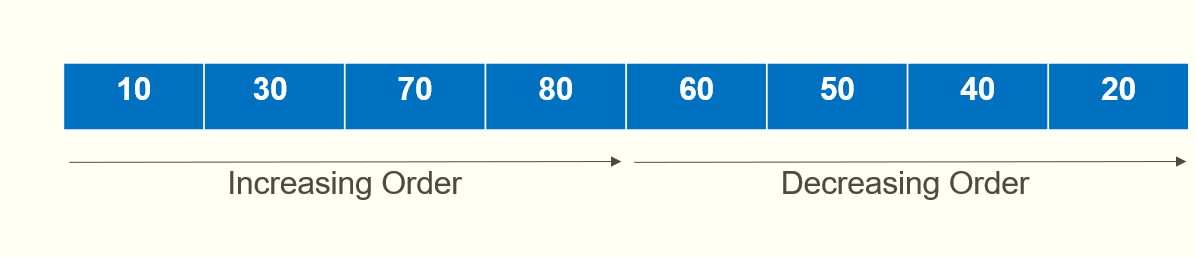
\includegraphics[width=8cm]{bitonic sequence.png} 
  \caption{Bitonic Sequence}
  \label{fig1}
 \end{figure}

\section*{Implementation}
For the implementation of the algorithm the problem can be broken into a series of nested finite state machines that control the state of the main sorting function. First there is one finite state machine to control the state of the entity as a whole. Such a machine would contain, at minimum, one state in which data is initialized into the entity or into memory, one state in which the sorting algorithm can operate, and one state in which the data is transferred out of the entity. The sorting state will then contain one finite state machine that controls the “Sort State” of the algorithm as shown in ``Fig.~\ref{figwiki}''. This finite state machine will contain \(log_2(Array Size)\) states. Each of these states will then contain a final finite state machine corresponding to each of the “Sub Sort States” shown in ``Fig.~\ref{figwiki}''. These machines will contain a number of states equal to the current “Sort State.” These states are all that is needed to create a well-defined entity that can be synthesized on an FPGA. Every state can then call a function taking the “Sort State” and “Sub Sort State” as its only inputs. If needed, a 3rd input can be defined as to whether the array is being sorted in increasing or descending order. Inside that function, parallel processes can be spawned corresponding to each of the elements that need to be compared and possibly swapped. For maximum time efficiency, one process will be spawned for every two elements in the array. Three tiers of parallel processes can define the items needed to be compared, each of these would correspond to a FOR loop in VHDL. The first tier takes only the “Sort State” as the input and creates \((Array Size)/(2^{Sort State})\) sub processes each corresponding to the blue and green boxes shown in ``Fig.~\ref{figwiki}''. \(2^{Sort State – Sub Sort State}\) processes will then be spawned in each of those processes. Each of those processes correspond to the red boxes in ``Fig.~\ref{figwiki}''. Finally, one process can be created for each of the lines shown in ``Fig.~\ref{figwiki}''. These processes must be aware of the corresponding number of the process tree that it is in. If numbering each process starting at 0, the compare and swap function must be called between the number of the current first process times two to the power of ”Sort state” plus the number of the current second process times two to the power of “Sub Sort State” plus the number of the current third process and the number two to the power of “Sub Sort State” elements above that. I.e. if the Sort State is 3, the Sub Sort State is 1, first process number is 1, the second process number is 2 and the third process number is 0 then the comparison is made between elements \(1*(2^3)+2*(2^1)+0\) and \(1*(2^3)+2*(2^1)+0+2^(1-1)\) (elements 12 and 13) in an array counting elements starting at 0. The comparison and swap will then ensure that the elements are in ascending order if the first process corresponds to a green box in the diagram or descending order if the first process corresponds to a blue box.
\begin{figure}[h!]
  \centering
  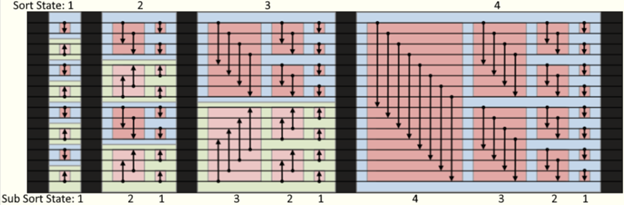
\includegraphics[width=8cm]{bitonic sorting.png} 
  \caption{Visualization of a 16 input Bitonic Merge Sort Algorithm with numbered Sort and Sub Sort States}
  \label{figwiki}
 \end{figure}


\section*{Results}
The results of implementing this code on an Artix-7 FPGA using Xilinx Vivado and VHDL code are as follows. The initialization of the array in memory and the reading of the sorted array from FPGA memory are highly dependent on the system interfacing with the hardware and therefore were not a focus of testing. These were done using the Vivado debugger. Where n is the number of elements in the array, the sorting algorithm is able to execute in exactly \((log^2_2(n) + log_2(n))/2\) clock cycles. On an Artix-7 with a clock speed of 450MHz, this code will execute in \(20/9*(log^2_2(n) + log_2(n))/2\) nanoseconds. A 32 element sorter would execute in 15 clock cycles (\(110/30\) nanoseconds) uses 9055 elements of the LUT and 1110 Flip Flops. The LUT will be the limiting factor as it grows at a rate of roughly 2.5x every 2x number of elements meaning that on an Artix-7 a max size of 128 elements can be sorted in one operation and any greater would need to be sorted as part of a larger sorting network. A design using fewer LookUp Tables at the cost of more Flip Flops would be able to handle a larger array at a time. Alternatively, a different FPGA or even an ASIC designed with a large LookUp Table would be able to handle larger arrays at a time.


\section*{References}


\begin{thebibliography}{00}
\bibitem{b1} K. E. Batcher, Sorting Networks and their Applications, Proc. AFIPS Spring Joint Computer Conference, 32:307-314, 1968.
\bibitem{b2} M. F. Ionescu and K. E. Schauser, "Optimizing parallel bitonic sort," Proceedings 11th International Parallel Processing Symposium, 1997, pp. 303-309, doi: 10.1109/IPPS.1997.580914.
\bibitem{b3} https://www.geeksforgeeks.org/odd-even-transposition-sort-brick-sort-using-pthreads/
\bibitem{b4}https://en.wikipedia.org/wiki/Batcher_odd%E2%80%93even_mergesort

\end{thebibliography}
\vspace{12pt}


\end{document}
